 \begin{center}
 \textbf{
 %\dots
\og 
Assomption : Marie élevée au ciel
 \fg{}
 %\dots
 }
 \end{center}

L'Assomption est un événement qui nous touche de près parce que l'homme est destiné à mourir. Mais la mort n'est pas le dernier mot.
Elle est comme nous le montre le mystère de l'Assomption. Le pape Pie XII, le 1er novembre 1950, dans la constitution apostolique \og Munificentissimus Deus\fg{}, déclare solennellement et défini que c'est un dogme divinement révélé :
\emph{\og Nous proclamons, déclarons et définissons que c'est un dogme divinement révélé que Marie, l'Immaculée Mère de Dieu toujours Vierge, à la fin du cours de sa vie terrestre, a été élevée en âme et en corps à la gloire céleste.\fg{}}
C’est pourquoi, elle a pu dire \og \dots Désormais tous les âges me diront bienheureuse\fg{}.
La Mère du Rédempteur a une place bien définie dans le plan du salut. Marie en tant que mère du Christ, est unie spécialement à l’Église. Elle garde fidèlement l’union avec le Christ. Ainsi ce "double lien" qui unit la Mère de Dieu avec le Christ et avec l’Église, prend une signification historique.
Il ne s’agit seulement de l’itinéraire personnel de sa foi et de la "meilleure part" qu’elle a dans le mystère du salut, mais aussi et surtout de l’histoire de tout le peuple de Dieu, de tous ceux qui participent au même pèlerinage de la foi.

L’Assomption ne veut pas dire que Marie n’est pas morte. Elle est morte comme toute personne humaine, comme Jésus lui-même est mort. Dans l'Église catholique, l'Assomption de la Vierge Marie est un dogme, c'est-à-dire une vérité de la foi qui fait autorité.
Marie élevée dans la gloire du Ciel nous attire et nous donne un avant-goût de cette joie éternelle promise par Dieu. Le 15 août est la grande fête religieuse de l'été et de la période des congés.
\begin{wrapfigure}{l}{1.0cm}
\vspace{-0.4cm}
	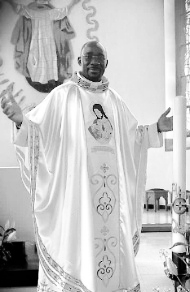
\includegraphics[scale=1.20]{../images/standing_daniel}
\end{wrapfigure}
Pendant nos vacances, arrêtons-nous pour réfléchir et célébrer la Vierge Marie.
Le 15 août nous rapproche de Marie et nous rappelle qu'elle veille sur nous chaque jour. Nous avons au Ciel une Mère qui intercède pour ses enfants.

La fête de l'Assomption élève notre esprit : Marie par son Assomption au Ciel est déjà ce que nous serons. Elle nous invite à nous élever spirituellement au-delà de nos préoccupations purement terrestres et à nous rendre attentifs aux valeurs importantes que nous négligeons souvent.
Aujourd’hui, notre regard doit s’élever vers le Ciel de toutes nos espérances.

\begin{flushright}
Bonne fête de l’Assomption à toutes et à tous !
\textit{Père  Daniel  ETTÉ}
\end{flushright}

